\subsection{Regional Data}
To analyse regional trends the dataset is segregated into sub-datasets for each of the 54 regions, and monthly total streams for all songs are aggregated. These songs are then arranged in descending order of their total streams across all months of the year, which reveals how the popularity of a song changes over the year in each region. To estimate a song's lifespan, we also rank the tracks according to how many streams they receive in each location throughout the year, along with the number of months they were in the charts. Out of the 54 locations, we discover that Ed Sheeran was the most listened artist in 33 regions, followed by J Baldwin in 10 and Ozuna in 4. "Shape Of You" was the only song that streamed across all regions the entire year.

\subsection{Audio Features}
The songs' 13 audio attributes are displayed separately to show the range of variation in their values (Appendix \ref{appendix:A}). We also plot a heatmap to look for correlations among them. It is noteworthy that the acousticness and energy of songs and the acousticness and loudness have a high negative correleation. Acousticness is a feature that represents how much of a song is produced using only acoustic instruments as opposed to electric or electronic ones. The category of soft emotional songs that are similarly characterised by low speechiness and danceability, are verified by this observation. Loud songs, namely dance or party tracks, are positively associated with more energy and danceability. However, these trends do not reveal how a song's attributes affect its global appeal.
\begin{figure}[h]
\centering
\centerline{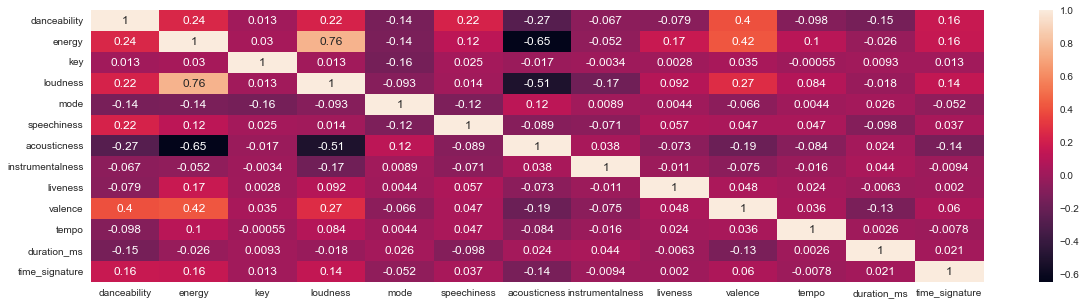
\includegraphics[width=\textwidth]{Outputs/Correlation Heatmap - Normalised Audio Features.png}}
\caption{Heatmap of correlations between the 13 normalised audio features}
\end{figure}

\subsection{Trends}
A time series analysis is performed exclusively on the  \textit{global} region of the dataset to see whether there is a weekly or monthly seasonality. Instead of analysing each region separately, the \textit{global} region is chosen because it compiles all listening trends worldwide. By adding up the streams of the top 200 songs for a given day, the global region data of the top 200 streams each day are transformed into the total number of streams per day. An additive model is used as the change in trend is independent of its value. We discover a weekly seasonality where the daily streams fluctuate on an average of 50,000 between weekdays and weekends after being broken down into trend, seasonality, and noise. This represents a 5\% fluctuation in the steams, and this finding indicates that, on average, people's listening preferences shift over the weekends.
\begin{figure}[h]
\centering
\vstretch{0.9}{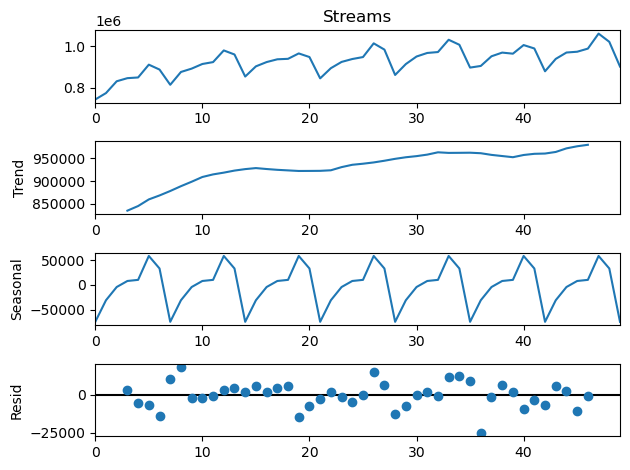
\includegraphics[width=0.5\linewidth]{Outputs/Trend.png}}
\caption{Seasonality of songs in the global region}
\end{figure}